\subsection*{Problem 23-1 Second-best minimum spanning tree}
\begin{enumerate}
	\item	Since a graph has a unique minimum spanning tree if, for every cut of the graph, there is a unique light edge crossing the cut(Exercise 23.1-6). Therefore, For a graph that all edge weights are distinct, the minimum spanning tree is unique. \\
		But the second-best minumum spanning tree need not be unique. Here is an example, \\
		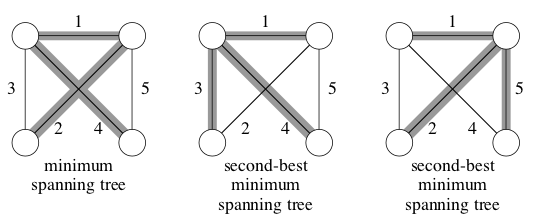
\includegraphics[width=10cm]{chapter23/second-best-mst.png} \\
	\item	只需要证明,若替换MST中的两条或两条以上的边,我们得不到一个Second-best Minimum Spanning Tree \\
		设$T$是图$G$的Minimum Spanning Tree,存在Second-best Minimum Spanning Tree $T'$,其中至少有两条边和$T$中不同;设边$(u, v)$是$T - T'$中权值最小的边,将边$(u, v)$加入$T'$中,则必然形成一个cycle,cycle中包含一些$T' - T$中的边$(x, y)$,则$w(u, v) < w(x, y)$ \\
		(若$w(u, v) > w(x, y)$,则将边$(x, y)$加入$T$,我们得到一个cycle,在cycle中包含一些$T - T'$中的边$(u', v')$,设$T'' = T - \{(u', v')\} \cup \{(x, y)\}$是一棵Spanning Tree,因为$T$是MST,所以$w(x, y) > w(u', v')$,即$w(u, v) > w(x, y) > w(u', v')$,与我们对于边$(u, v)$的选择矛盾) \\
		所以对于Spanning Tree $T' - \{(x, y)\} \cup \{(u, v)\}$,其权值比$w(T')$小,且其和MST $T$不同,即$T'$不是Second-best Minimum Spanning Tree
	\item	For each vertex $u$, using DFS to find $\max[u, v], v \in V$. The running time is $\mathcal{O}(V^2)$
	\item	\begin{enumerate}
			\item	Find Minimum Spanning Tree of $G$........$\mathcal{O}(E + V \log V)$
			\item	Compute $\max[u, v]$ for all $u, v \in V$........$\mathcal{O}(V^2)$
			\item	Find an edge $(u, v) \notin T$, that minimizes $w(u, v) - w(\max[u, v])$........$\mathcal{O}(E)$
		\end{enumerate}
		The Second-best minimum spanning tree is $T - \{\max[u, v]\} \cup \{(u, v)\}$ \\
		The running time of the algorithm is $\mathcal{O}(V^2)$
\end{enumerate}

